\documentclass[10pt,twocolumn,letterpaper]{article}

\usepackage{cvpr}
\usepackage{times}
\usepackage{graphicx}
\usepackage{amsmath}
\usepackage{amssymb}

% Include other packages here, before hyperref.

% If you comment hyperref and then uncomment it, you should delete
% egpaper.aux before re-running latex.  (Or just hit 'q' on the first latex
% run, let it finish, and you should be clear).
%\usepackage[pagebackref=true,breaklinks=true,letterpaper=true,colorlinks,bookmarks=false]{hyperref}

\cvprfinalcopy % *** Uncomment this line for the final submission

%\def\cvprPaperID{****} % *** Enter the CVPR Paper ID here
%\def\httilde{\mbox{\tt\raisebox{-.5ex}{\symbol{126}}}}

% Pages are numbered in submission mode, and unnumbered in camera-ready
\ifcvprfinal\pagestyle{empty}\fi

\begin{document}

%%%%%%%%% TITLE
\title{Class-Specific Object Segmentation using Top-Down Attribute Support}

\author{Aron Yu\\
Department of Electrical Engineering\\
University of Texas at Austin\\
{\tt\small aron.yu@utexas.edu}
\and
David J. Garcia\\
Department of Computer Science\\
University of Texas at Austin\\
{\tt\small djchooy@utexas.edu}
}

\maketitle

%%%%%%%%% ABSTRACT %%%%%%%%%
\begin{abstract}
 Object localization and image segmentation can be considered as part of the same problem: dividing up an image in a meaningful way.  However, there is a ``semantic'' gap between top-down semantics and bottom-up segmentations.  Top-down approaches attempt to detect objects and to fit object-specific templates/statistics to image regions.  Bottom-up approaches use local features to inform the segmentation by joining groups of similar pixels.  In our approach, we use learned attributes to aid a bottom-up segmentation engine.  Using attributes enables us to apply our method to a variety of object classes, including ones not present during attribute training.  While some approaches consider bottom-up segmentation as a ``preprocessing'' step in a segmentation pipeline, we perform the segmentation while considering detected attribute locations.  We show significant improvement over a bottom-up baseline segmentation routine.
\end{abstract}

%%%%%%%%% INTRODUCTION %%%%%%%%%
\section{Introduction}
Semantically, it's intuitive to describe objects by their attributes.  Describing objects by their attributes has the additional benefit of extending, not only across members in the same object categories, but also across the categories themselves \cite{Farhadi2009}.  For example, members of the categories ``Farm Animals'' and ``House Animals'' both have the ``Legs'' attribute.  This idea might provide valuable context to the task of both object presence detection as well as object segmentation in an image.  It may be possible to, without knowing the category, describe an object with its attributes and potentially localize it in an image.

However, it is important to keep in mind that each object category has its own distribution of attributes.  Horse and sheep have ``Legs'', for example, but unlike a sheep, a horse is not ``Fluffy''.  Likewise, a wooden cart and a car both have ``Wheels'', but the wooden cart is not ``Shiny''.  These problems can be mitigated with strong negative examples in training \cite{Farhadi2009,Farhadi2010}.

Another potentially complicating factor is the ``Semantic Gap'' between image content and the semantic meaning of that content \cite{Ma2007}.  For example, suppose the category ``Bear'' has two types of attributes: ``Fuzzy'' and ``Eats Fish''.  The former attribute can be easily represented with a texture (a mid-level feature).  The latter, however, is very difficult to represent with either low-level features.  Typically, these types of problems are only tractable as a discriminative learning problem with a respective positive/negative training-set.

\begin{figure}[t]
\begin{center}
    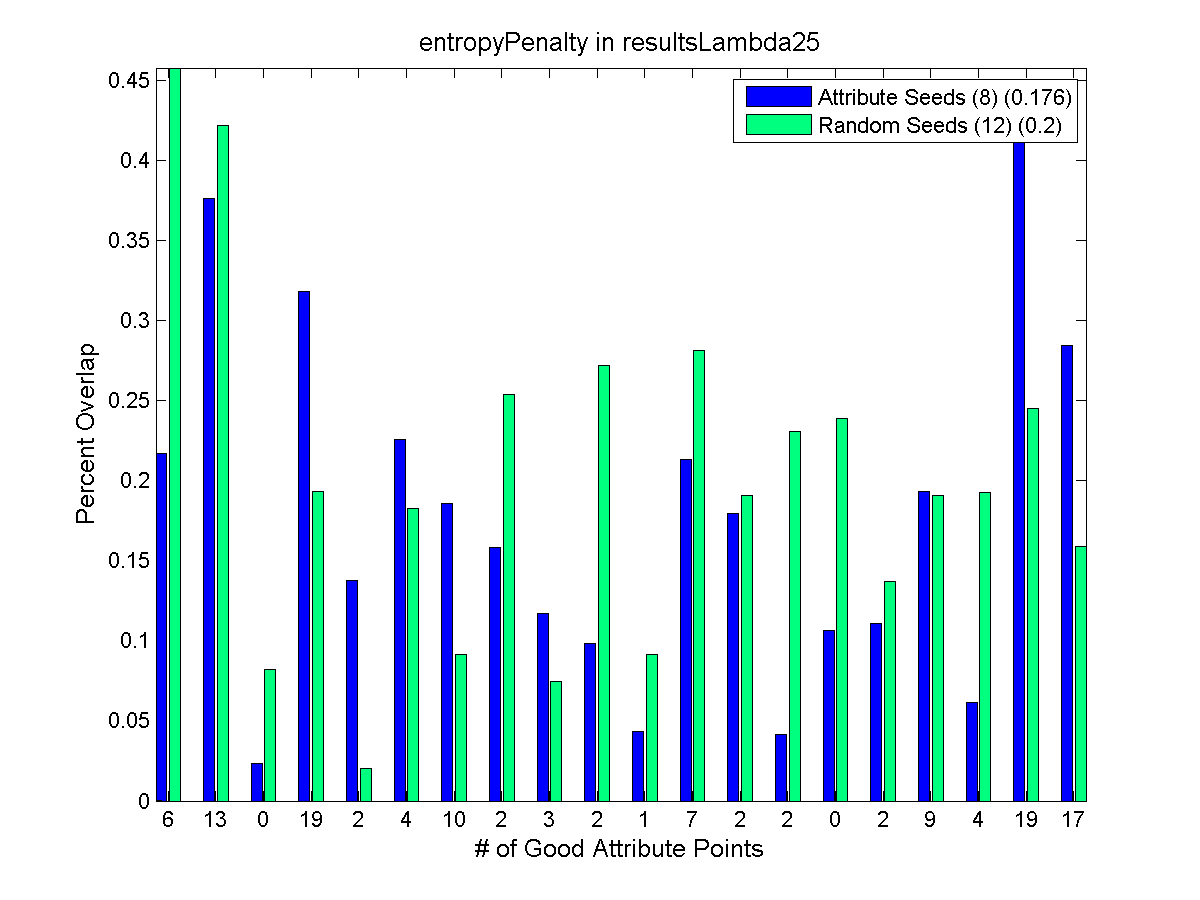
\includegraphics[width=0.9\linewidth]{carscore}
\end{center}
\caption{Overview of our complete pipeline. Given the semantic attributes of the object of interest, identify the key attribute points and use them as seed points for segmentation.}
\label{fig:overview}
\end{figure}

The typical end game motivation for these types of tasks is to accurately, and precisely, segment object(s) of interest in images.  There are various applications for this capability.  Obviously, knowing \textbf{where} an object is, in an image, is related to knowing that an object is present in the image in the first place.  Said another way, knowledge of object presence is a necessary, but not sufficient, condition for object localization.  Object tracking, for example, requires extraordinarily precise location information \cite{Choi2012}.  Likewise, scene understanding benefits enormously from localization of constituent objects.  A ``gathering'' activity necessarily requires knowledge of individual person locations in order to infer that they are converging on a central location.

Many object localization techniques have a pipeline that starts with low-level segmentation to produce superpixels.  Top-down information, usually obtained from a trained classifier, associates these mid-level features with each other to produce a final segmentation.  The initial segmentation is little more than a preprocessing step: a process to produce a higher level feature that is easier to work with.  This approach has the obvious advantage of not having to rely on some trained machine to do the low level processing.  We investigate how one could use top-down information in this initial preprocessing step.  Specifically, we look at how attribute location priors could inform bottom up image segmentation.  We adapt the bottom-up parametric graph cuts technique to take into account the color distribution indicated by the attribute locations in the image \cite{Boykov2001}.  Given good attribute location priors, we feel that an initial segmentation can be significantly improved.  We also demonstrate the degradation in performance as attribute accuracy degrades respectively.

\section{Related Works}
Our approach is the most similar to \cite{Carreira2010}.  We investigate modifying the data-cost term by incorporating the location of detected attributes.  Unlike the authors in \cite{Carreira2010}, we propose that foreground seed placement can have a significant impact on the initial segmentation results.  The work done by \cite{Gould2010} classifies superpixels based upon relative location priors of the objects in the images.  For example, if ``Cows'' are typically $above$ ``Grass'', then there is a relatively high probability that a cow will be above grass in an image.  Relative location priors are taken into account after superpixels are ``initially'' classified using lower level features.  Essentially, the location priors are a refining technique.

In the work done by \cite{Farhadi2009}, the authors observe the potential for attributes to cross categories and thus suggest that a general classifier can be built with minimal training.  \cite{Farhadi2009} also distinguish between semantic attributes and discriminative attributes.  The former captures ideas like shape (``boxy'', ``cylindrical''), part (``has head'', ``has leg''), and material (``has wood'', ``is furry'').  The latter type of attributes is meant to enable discrimination between classes.  Cats and dogs, for example, have many common semantic attributes.  These attributes represent splits that effectively split classes from each other.  In the work of \cite{Berg2012}, the authors show that there are important ``Compositional Factors'' that can bias where salient objects are in the image.  \cite{Berg2012} considers compositional factors to be the size and location of the salient object.  Since our experimental goal is to essentially infer a foreground in images, our task is not unlike the task in \cite{Berg2012}.  We simply use a standard color distribution for our features.

Of special note is the work of \cite{Boykov2001}.  The authors model image segmentation as a four-way graph cut problem with respect to K number of classifications any one pixel can take.  The choice of pixel classification is essentially reduced to min-cut/max-flow problem.  The optimal classification is the one that results from removing links that, when added together, have the lowest energy possible.  Also of note in this work is restriction on the data cost function  $D_p$.  This function captures how well the label $f_p$ fits label $p$ given the observed data.  In our case, the observed data is simply the color of the pixel with respect to foreground and background color distributions. The entire energy function that is to be minimized is of the form:
\begin{equation}
\textrm{E}(f^C)  =  \sum_{p \in \textrm{P}}{D_p(\textrm{$f^C_p$}) } + \sum_{\{p,q\} \in \textrm{N}}{V(f^C_p,f^C_q)}
\label{eq:energy}
\end{equation}
$f^C_p$ is the label that we give to pixel $p$ for the minimal graph cut $C$.  $V(f^C_p,f^C_q)$ is the function that describes the pairwise labelings between any two pixels $p$ and $q$.  It is understood that $N$ only contains edges between adjacent pixels.

%%%%%%%%% ATTRIBUTES %%%%%%%%%
\section{Top-Down Attributes}

Explain how we're using attributes
- trained attribute detectors causes pixels to respond
- cluster the pixels into key attribute points


\subsection{Attribute Detectors}

Talk about the attribute detector from the Farhadi paper.
- works pretty well on localized objects, finding unusual attributes, etc
Briefly talk about the base features and the semantic features used
- attempt at avoiding attribute transfer

Manually selected the attributes for each class
- picked only semantic attributes
- list out the attribute for each class (maybe a table) with reference to the dataset section


\subsection{Attribute Points}

Back traced the locations of each attributes
- minor details about down sampling the color features to be fair
Clustering the feature locations
Show good sample images of the back traced features
Note that the detectors are not meant for localization
- divided into grids that suppose to benefit from object placement
- trained on localized objects
- talk about dominance of the color features

Simply took the raw result points from the attribute detector and tried to detect without using part detector like \cite{Farhadi2010}.

Measure the quality of attribute localization by counting the number of dots that lands on the objects.


\subsection{Performance}

Show images of the attribute points
Problems with approach, no the best
- not completely decoorelated but we can deal with the result since we're not looking for perfect localization

Show images of objects detected using wrong set of attributes




\begin{figure}[t]
\begin{center}
    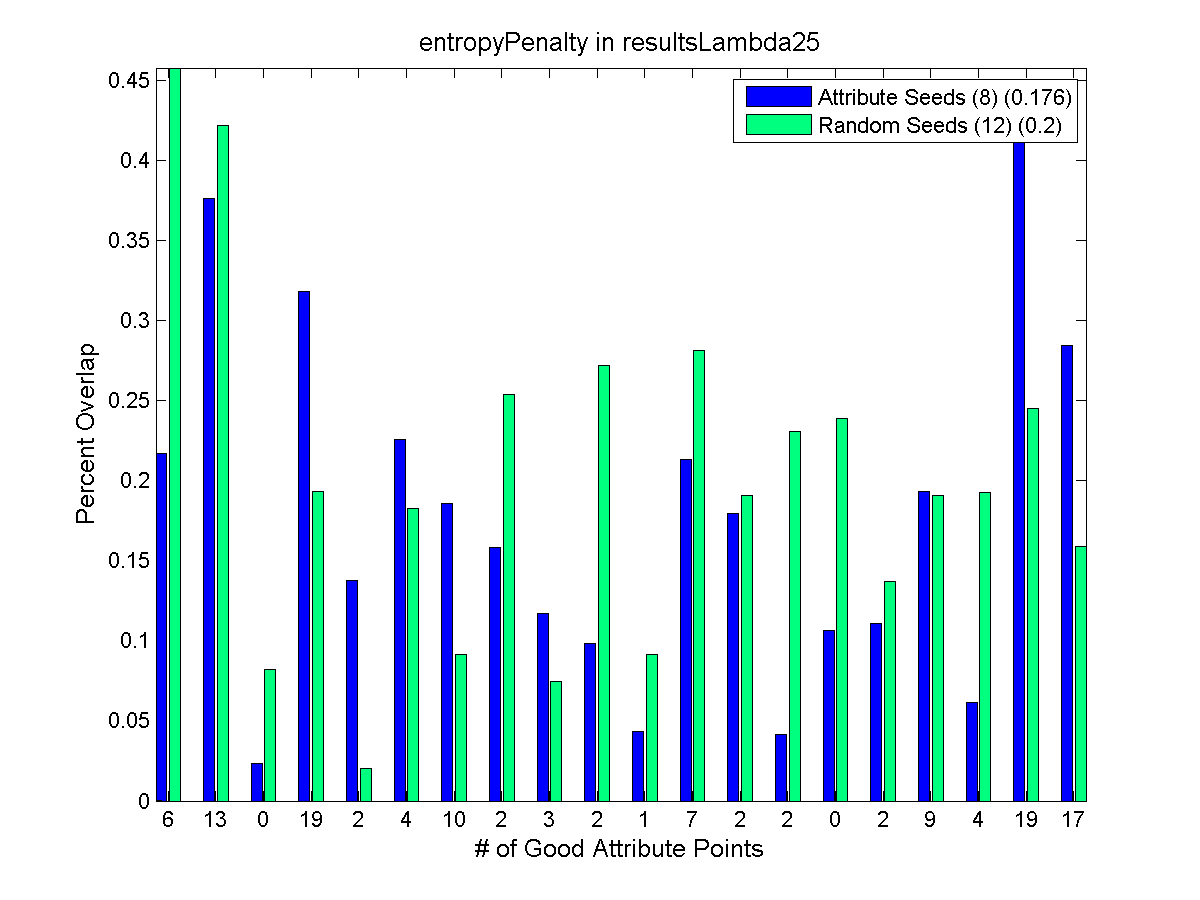
\includegraphics[width=0.9\linewidth]{carscore}
    \caption{Scores for Cars using a bias of 25.}
\end{center}
\label{fig:scores}
\end{figure}

%%%%%%%%% SEGMENTATION %%%%%%%%%
\section{Bottom-Up Segmentation}

Use seeds as starting point


\subsection{Graph Cut}
In section \textbf{1.1} we briefly discuss the minimization of

\[
\textrm{E}(f^C)  =  \sum_{p \in \textrm{P}}{D_p(\textrm{$f^C_p$}) } + \sum_{\{p,q\} \in \textrm{N}}{V(f^C_p,f^C_q)}
\]
For simplification, the main component of the pixel classification cost is a weighted difference in the probability that the pixel belongs to the foreground versus the background.  Since we only have these two classes (i.e. foreground and background), we only have to define two class weightings.
\begin{displaymath}
	\textrm{$D^c_p$}(p) = \left\{
		\begin{array}{lr}
			\inf & : p \in bgSeeds ,  c = foreground\\
			\textrm{$\mu_f$} & : p \notin bgSeeds,  c = foreground\\
			\inf & : p \in fgSeeds,  c = background\\
			\textrm{$f(p) + \lambda$} & : p \notin fgSeeds,  c = background
		\end{array}
	\right.
\end{displaymath}

\[
\textrm{f}(p) = \textrm{$P_\textrm{$fg$}$}(p) - \textrm{$P_\textrm{$bg$}$}(p)
\]		 

Function $f$ is the simple difference in probabilities between a pixel $p$ belonging in the foreground versus the background.  There are a couple versions of this cost function that we evaluate.  Essentially, however, the other functions are simply weighted versions of this function.

$\mu_f$ is the average difference between the probability of foreground membership versus background membership.  This strategy was partially informed with experimentation, but it functions as a naturally neutral cost value for the statistics of any one image.

$V$ is simply the location variant gradient smoothness of the image.  In other words, $V(p,q)$ is high if there is a large gradient difference between $p$ and $q$.  $V$ is location variant in the sense that this cost is obviously different between different sets of pixels.  In \cite{Boykov2001} there is a version of $V$ that maintains the same cost for all pairs of pixels.

Explain the use of Graph Cut for segmentation
- use of starting seeds, obtaining foreground/background color histogram
- various biases


\subsection{Cost Functions}

The formation, rationale behind our choices

Sample Equation
\[
\textrm{L2 Score} (u_s) = T_s\bigg[ \sum_{k \in \textrm{followers}}{P(\textrm{$u_s$ influences $u_k$})} \bigg]
\]


\subsection{Raw Segmentation}

not doing ranking and fast elimination
sample images of the segmentation results


%%%%%%%%% EXPERIMENTS %%%%%%%%%
\section{Experiments}

Testing with 3 data cost functions and 4 background bias values for each class and then compute the overlapping score with ground truth
Trying to see how "good" attribute points can help with segmentation


\subsection{Dataset}

Used VOC2008 dataset (cite the dataset)
- because that's what the attribute detectors were trained on
- used the segmentation dataset as testset due to the availability of ground truth
- tried to pick ones with only 1 class in the image
- formed a smaller 6-class dataset with 20 images per class


\subsection{Score Evaluation}

Compute the overlap score, intersection over union, of the segmentation and the GT
Since we don't have perfect segmentation, we look at the relative performance

Bulk of the discussion
- compare the 12 sets of results, which one is better, why and why not, etc
- show score bar graph comparison
- consider the number of "good" attribute points



\subsection{Extra Cases}

\textbf{Good Attributes}

Manually select the images that achieved good attribute points from all classes
- evaluated the overall result


\textbf{Multiple Objects}

Tried with images containing multiple objects just to see result
- objects from different classes


\begin{table}
\begin{center}
\begin{tabular}{|l|c|}
\hline
Method & Frobnability \\
\hline\hline
Theirs & Frumpy \\
Yours & Frobbly \\
Ours & Makes one's heart Frob\\
\hline
\end{tabular}
\end{center}
\caption{Results.   Ours is better.}
\end{table}

\section{Discussion}

conclusion
- we've shown that good attribute points leads to better segmentation
- better attribute detector would lead to better results

future work
1) Better attribute detector
2) Try cross-category generalization
3) Implement the full system
4) Try different cost functions, besides color histogram
5) Retrain attribute detector with less inter-class correlation


%-------------------------------------------------------------------------
\subsection{Illustrations, graphs, and photographs}

All graphics should be centered.  Please ensure that any point you wish to
make is resolvable in a printed copy of the paper.  Resize fonts in figures
to match the font in the body text, and choose line widths which render
effectively in print.  Many readers (and reviewers), even of an electronic
copy, will choose to print your paper in order to read it.  You cannot
insist that they do otherwise, and therefore must not assume that they can
zoom in to see tiny details on a graphic.

When placing figures in \LaTeX, it's almost always best to use
\verb+\includegraphics+, and to specify the  figure width as a multiple of
the line width as in the example below
{\small\begin{verbatim}
   \usepackage[dvips]{graphicx} ...
   \includegraphics[width=0.8\linewidth]
                   {myfile.eps}
\end{verbatim}
}

%%%%%%%%% REFERENCES %%%%%%%%%
{\small
\bibliography{attributebib}
\bibliographystyle{ieee}
}

\end{document}
